\chapter{Discussion}\label{ch5}
\newpage

\section{Thesis synthesis}
This thesis provides the initial development and implementation of a new modelling framework integrating macro-economic, land-use and biodiversity modelling to assess the impacts of future socio-economic change on global biodiversity.
The first iteration of our framework was a continental-scale assessment of synergistic climate and land-use impacts on more than 1000 bird species (\Cref{ch2}). With this work we showed that assessment of multiple socio-economic and biophysical drivers of biodiversity at very fine resolutions are feasible with modest computational and modelling infrastructure and expertise.. This initial work unraveled some of the complex pathways through which climate change impacts biodiversity, including through direct biophysical changes and through changes to global commodity demand and supply. This demonstrated the utility of integrated assessment frame- works to simultaneously analyze multiple drivers, and improve predictions of biodiversity change. A crucial outcome was the identification and prioritisation of research priorities, in particular (i) improving our ability to predict land-use change in response to commodity demand change, (ii) making predictions at a global scale to better capture global exports of biodiversity impacts, (iii) parametrizing scenario assumptions in line with established future narratives \citep[the so-called ‘shared socio-economic pathways’][]{oneill_new_2014}, and (iv) increasing the taxonomic scope of our biodiversity predictions to generalize biodiversity predictions (see \Cref{ch5:fig1}).


\begin{figure}[htb]
\centering
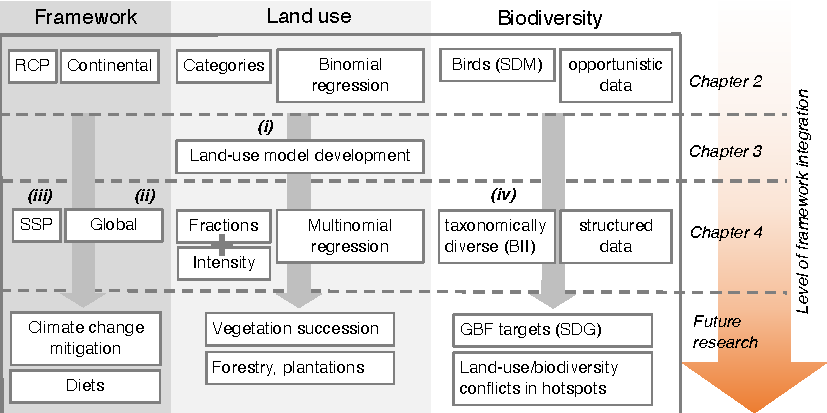
\includegraphics{chapters/figures/chapter5/fig1.pdf} 
\caption{Overview of developments accomplished in terms of scenario development, land-use and biodiversity modelling throughout this thesis. The second chapter identified research priorities (i-iv) that were tackled in subsequent chapters.}
\label{ch5:fig1}
\end{figure}

\subsection{Improving the land-use change model (i)}
\label{ch5:section_lumodel}
Following our initial study, we identified that the accessibility of our framework continued to be limited by the high parametrization requirements of the applied land-use model CLUE-S \citep{verburg_modeling_2002}. In CLUE-S, land-use elasticities (the propensity of land-uses to shift across the landscape in response to bottom-up processes, without changes to the overall occupied areas) are predominantly subjectively estimated. In addition, land-use suitability in the model is described using independent regression models for each land-use type, rather than allowing suitability to also be conditional on the predicted suitability of other land uses. The model is also limited by predicting fixed land-use categories, even though literature suggests that the fitting of downstream ecological models can be improved by using fractional land-use data, because fractional representations of land-use provide a higher level of sub-pixel information  \citep[\Cref{ch3}][]{bevanda_adding_2014, levers_drivers_2014, levers_drivers_2016}. 

To address these short-comings, we developed a bespoke land-use model in \Cref{ch3} ('FLUTES'). We implemented our land-use model fully in the 'R' programming language \citep{r_development_core_team_r_2008}, thus ensuring accessibility for R-trained ecologists. Our land-use model implements land-use fractions to bring the representation of land-use further in line with the optimal requirements for downstream ecological models. We also developed a multinomial suitability model in which land-use suitability is modelled conditional on the suitability predicted for other land-use classes, thus implicitely providing parametrization of bottom-up processes affecting the location and magnitude of land-use change (competition between land uses). Compared to our implementation of Dyna-CLUE, our model also improves the parametrization of land-use elasticity by using observed data to determine locations where a new land-use can be established without having been present historically.

\subsection{Increasing the spatial extent of analyses (ii)}
In \Cref{ch4} we provided a first global implementation of our framework and compared biodiversity change predictions made using our comparatively simple and streamlined framework to those provided by a large integrated assessment framework known as ‘Message 8.5’ \citep{riahi_rcp_2011}. Following an analysis pathway provided by \citet{newbold_global_2015}, we generated economic demand, land use and biodiversity predictions using with our intertemporal GTAP model ’GTAP INT’ and our land-use model ’FLUTES’. We then compared the biodiversity predictions derived using the two framworks. Global predictions of agricultural land-use demands and their spatial realisation were predicted to be similar between the models, even though some more work is required to appropriately model and evaluate spatial predictions of primary and secondary forest habitats (see \Cref{ch5:section_lumodel}). Despite  this caveat, we were able to bring our framework to the global scale and found a comforting congruence of predictions, despite the fact that our model is far more streamlined, pattern-based and simple to use. This finding confirmed that our streamlined approach with minimal parametrization requirements is a potent tool that may allow IAM to be more widely used by a greater variety of agencies and organisations that seek integrated analysis of biodiversity outcomes in complex socio-ecological contexts.


\subsection{Scenario alignment (iii)}
In \Cref{ch4}, we further aligned our scenario parametrization with the SSPs \citep{oneill_new_2014} and provided the foundation for detailed assessments of climate change mitigation and trade. Using GTAP INT, we parametrized RCP8.5 with environmental damage functions. Since RCP forcing levels are emergent properties of SSPs, we assumed that our projection of economic damages under a given RCP approximates economic damages we would expect under a related SSP, also assuming that aspects of socio-economic change, such as gross domestic product (GDP) and population growth, are implicit in this parametrization. This assumption was necessary because adjusting population growth and GDP explicitly is not possible in GTAP INT. However, in our GTAP INT implementation, we applied climate damages of RCP 8.5 in order to approximate SSP 5 and achieved similar predictions for agricultural land demand as predicted by Message 8.5. This suggests that our framework provides good approximations of predictions made under established harmonized scenario assumptions. The GTAP INT model we applied in Chapter 4 is also an improvement over the GTAP INT model we applied in \citet{kapitza_assessing_2021} (\Cref{ch2}). In the previous iteration, we assumed a linear temperature increase to levels that correspond with scenarios we explored (RCP 2.6 and and RCP 8.5). In the more recent iteration, we directly included temperature trajectories as they were predicted for the RCP under the MAGICC6 model, without requiring linear interpolation. This results in a more realistic representation of future economic damages.

When analyzing other aspects of socio-economic change, it is crucial to account for RCP, population growth and GDP independently, because climate change mitigation strategies may lead to different combinations of socio-economic change with radiative forcing. For example, when the global policy response to mitigate climate change is highly fragmented, mitigation costs are high regardless of GDP and population growth, making it less likely that reductions in forcing levels and warming can be achieved \citep{kriegler_fossil-fueled_2017}. Accordingly, in order to explore scenarios of global climate change mitigation, RCP cannot always be used as a proxy for SSP and further scenario parametrizations will usually be necessary to properly parameterize an SSP.


\subsection{Increasing taxonomic scope (iv)}
In the initial iteration of our framework we applied models based on presence-only data, because these data are widely collected in opportunistic surveys and collated through the Global Biodiversity Information Facility (GBIF) data base, making them readily available for modelling studies \citep{gbif_gbif_2016}. However, as for most other biodiversity data sampled in unstructured surveys, sampling bias remains a pervasive issue undermining the vast geographic, temporal and taxonomic coverage of the data base \citep{troia_filling_2016, kapitza_assessing_2021}. Even though methods exist to account for sampling bias, they tend to depend on the study context and lack coherent approaches that can be scaled up \citep{kramer-schadt_importance_2013, stolar_accounting_2015, kapitza_assessing_2021, fithian_bias_2015}.

Our applied species distribution models required at least 20 occurrence points to estimate relative likelihoods of occurrence and applying this filter for the countries chosen in the analysis, the only taxonomic group with sufficient (\(>\)1000) species satisfying this requirement was birds. An additional advantage of using bird species was that we could make simple assumptions about the realisation of predicted potential niches, because the ability to fly implies relatively unconstrained dispersal (we only constrained dispersal in Australia to adjacent bioregions) \citep{kapitza_assessing_2021}.

Changes in the geographic distributions of birds alone give an insufficient picture of biodiversity and the continental scope of the initial study limits the generalisation of findings to global geographic extents. To be able to assess human impacts on biodiversity at a global scale, it is necessary to maximise the representation of taxonomic diversity, because impacts are heterogeneous across taxonomic groups \citep{hudson_predicts_2014}. Our GBIF-based method of stacking SDM applied in \Cref{ch2} would have quickly caused data processing and modelling requirements to exceed the computing power available to me, given that the GBIF data base currently holds almost 1.5 trillion records for Animalia alone \citep{gbiforg_gbif_2021}. Given that we ran continental-scale SDM for bird species on a high-performance cluster on 12 parallel cores and these computations took approximately 72 hours to complete, significant computational challenges would also have arisen during model building and prediction when upscaling the analysis to all taxa and to a global extent. 

Several authors argue for the additional benefits of using abundance-based metrics to evaluate biodiversity change \citep{scholes_biodiversity_2005, newbold_global_2015}.

To overcome these barriers, we based our biodiversity models on structured survey data from the PREDICTS data base. The PREDICTS data base allows for the calculation of macroecological indices that are based on effort-corrected abundance measures from structured surveys that cover 13 out of 14 biomes, 25 out of 35 biodiversity hotspots and 28000 species from various taxonomic groups, including plants, insects, amphibians, mammals, birds and reptiles. For our research priority of providing global predictions of biodiversity change, the data base provides an ideal alternative to GBIF, because quality-control and bias-accounting are part of the data collection and submission protocols \citep{hudson_predicts_2014}. With PREDICTS, we were quickly able to estimate and predict biodiversity intactness \citep{scholes_biodiversity_2005}, providing a simple approach to estimate a response of biodiversity to scenarios of socio-economic change with global coverage, accounting for both species richness and abundance. As the name suggests, the biodiversity intactness index provides an overall index of how biodiversity is anticipated to change with broadly changing land-use patterns.  The properties of the index have not been widely tested or evaluated against observed species level change in a variety of landscapes. There exists an opportunity to compare how a biodiversity intactness index analysis compares with an analysis of change based on species distribution models.

\section{Opportunities for improvement}

\subsection{Improving the biodiversity intactness model}
BII is a general index that cannot account for all important aspects of biodiversity change. A fundamental limitation is the exclusion of species-level information when estimating the underlying macroecological indices (abundance and similarity) from which BII is calculated. When this information is missing, it is not possible to track the status of endangered species. For example, this could lead to predictions of high intactness in biodiverse regions, where human impacts have historically particularly affected endangered species that already have experienced abundance declines. While impacts on these species may have been severe, they are not represented in BII \citet{martin_biodiversity_2019}. To predict localized impacts on many endangered species and derive optimal conservation policy, species distribution models are better suited because they can capture fine-scale variations in environmental space. Predictions of habitat suitability typically provided by SDM allow for the spatial prioritization of areas for conservation and restoration \citep{wilson_applying_2011}. The systematic selection of a small number of flagship species can even be an effective tool for efficient conservation prioritization representative of global biodiversity \citep{mcgowan_conservation_2020}.

Another limitation to the estimation of BII from the PREDICTS data base is posed by its reliance on a relatively coarse representation of land-use. \citet{martin_biodiversity_2019} critisized that global intactness trends predicted by \citet{newbold_global_2016} likely underestimated historic losses of biodiversity in tropical plantation forests and dense population centers, and overestimated biodiversity declines in semi-arid rangelands. Spatial patterns of biodiversity intactness and biomass intactness \citep{erb_unexpectedly_2018} can be expected to correlate in space. However, \citet{martin_biodiversity_2019} found that spatial patterns in these indices did not agree for many parts of the world, even exhibiting a strong negative correlation when measured across 32 biodiversity hotpots. Significant improvements to our framework may be achieved by matching land uses recorded in the PREDICTS data base to the more highly resolved Land Use Harmonization Project 2 (LUH2) database \citep{hurtt_harmonization_2020}. In LUH2, rangeland and pastureland are distinguished, allowing for a more discriminate modelling of the biodiversity response to these classes. Furthermore, superimposing global plantation maps \citep{harris_spatial_2019} would allow a much more discriminate mapping of forest types that each differ in their implications for biodiversity. Including adequate global land-use maps that are precise in terms of distinguishing habitats of different significance for biodiversity should remain a high priority in future developments of our framework, regardless of the applied biodiversity models.


\subsection{Improving FLUTES}

The approach to model land-use change we provide through our FLUTES model is based on statistical regression analysis and a simple allocation algorithm. We intentionally simplified our model to streamline parametrization requirements for the application in global biodiversity assessments (\Cref{ch3}). However, rangelands and pasturelands, as well as natural forests and plantation forests, are often observed within the same environments \citep[for example, semi-arid rangelands and pasturelands on the Australian continent, or natural forests and plantations in tropical regions, see][]{newbold_reply_2019}. Basing a land-use model almost entirely on regression methods (as done in FLUTES) that model observed patterns (including transitions) limits the ability of FLUTES to represent bottom-up processes that drive fine-scale land-use change patterns \citep{noszczyk_review_2019}. FLUTES could be made arbitrarily more complex and include arbitrarily many land-use classes and variables that predict their suitability. The challenge is finding the right level of complexity for the problem at hand. If a very fine-scale analysis of local land-use changes is required, it may be better to use a more mechanistic model such as LUTO \citep{bryan_supply_2014}, so that complex human behaviours that influence land-use change can be incorporated and analyzed.

Advances in computational capacity have increasingly allowed for the application of machine learning techniques, such as Artificial Neural Networks (ANN) in land-use change modelling \citep{noszczyk_review_2019, koomen_core_2011}. ANN are powerful tools to recognize patterns of change from observed land-use time series. They apply user-defined transition rules and predict transitions based on the relationship of historic land-use change patterns with a wide range of socio-economic and biophysical variables \citep{pijanowski_using_2002}.  The main advantage of ANN over our method is that finely resolved spatial information from entire historic time-series can be used to train networks. FLUTES also uses historic land-use time series, but the information is only used to constrain the model by limiting how much of a land use can be established where it was not historically present. This provides a less refined parametrization of the magnitude and location of transitions between land-uses through time, because observed spatial patterns are not taken into account.

Despite their advantages, ANN are also somewhat limited because they simulate and predict categories of land use. In order to achieve an information content in the final land-use map that at least matches the fractional maps produced by FLUTES (currently at 10km), predictions at an even higher spatial resolution of \(>\)10km would be required, possibly leading to computational and data constraints at the global scale. ANN are also limited by 


Nevertheless, given the fine-scale dynamics of land uses that drive species habitat change and, consequently, biodiversity intactness, unsupervised learning methods that use historic land-use time series, such as ANN, are likely to significantly boost our framework's predictive capacity.

\subsection{A streamlined and open integrated assessment framework to predict biodiversity}

The work in this thesis was driven by the need for integrated, cross-disciplinary approaches to biodiversity modelling \citep{ipbes_summary_2016, ipbes_summary_2019}. 

Established integrated assessment models (IAM) are typically designed for the assessment of economic transformation strategies to mitigate and adapt to climate change and as such provide little to no insight on biodiversity outcomes \citep{harfoot_integrated_2014}. In addition, by applying highly parametrized submodels that are developed and maintained by large research teams and backed through institutional support, they are prohibitively complex in an ecological research context. For this reason, adopting existing IAM for biodiversity assessments continues to be faced with significant barriers. 

Despite these limitations, biodiversity assessments applying at least some degree of cross-disciplinary model integration have been implemented recently, also including the first case study of this thesis \citep[\Cref{ch2},][]{kapitza_assessing_2021}. \citet{newbold_global_2015} provided a spatially-explicit assessment of global biodiversity intactness under future land-use changes predicted under the Message 8.5 model \citep{riahi_rcp_2011} and \citet{marques_increasing_2019} applied economic and land-use models to identify the extent to which economic teleconnections have led to remote, exported impacts of economic activity on avian diversity globally. More complete levels of integration between economic, land-use and biodiversity modelling have been provided by \citet{leclere_bending_2020}, who use the land-use modelling components of several IAM to examine how to halt and reverse the decline of terrestrial biodiversity while simultaneously growing sufficient food for the world's growing human population. \citet{veerkamp_future_2020} use two established IAM to predict biodiversity and ecosystem services in a European context. \citet{kapitza_assessing_2021} assess biophysical and socio-economically mediated climate change impacts on bird species at continental scale, by coupling a general equilibrium model with land-use and biodiversity models (\Cref{ch2}). 

Nevertheless, such examples of integrated biodiversity assessments remain rare and they also continue to be limited by their scalability to global extents, their coarse spatial resolutions preventing adequate representation of highly localised processes, and the extent to which their scenario assumptions are aligned with socio-economic narratives applied in other disciplines, such as climate science. Addressing this gap, we designed our framework to be accessible in ecological research environments, ensure high spatial resolutions at global scales and align model assumptions with future narratives already established in the IAM community.

Our framework also attempts to address the reproducibility crisis in science \citep{open_science_collaboration_estimating_2015}, which also affects ecology as a discipline \citep{fidler_metaresearch_2017, fernandez-juricic_why_2021}. We coded and documented our methods to model land-use and biodiversity change fully in \texttt{R} \citep{r_development_core_team_r_2008}, thus making our code accessible to a fast growing number of ecologists trained in R: \citet{lai_evaluating_2019} found that the share of studies published in 30 ecology journals that report \texttt{R} as primary tool for analysis has increased from 11.4\% in 2008 to 58\% in 2017, also highlighting the importance of \texttt{R} as a catalyst for open science and reproducibility. Our implementation of GTAP INT does not yet interface with R, but according developments are currently underway.

Moreover, our framework parametrization makes assumptions that significantly streamline the analysis and provide substential reductions in model complexity compared to established IAM. For example, we linked 8 crop sectors to one cropland class and used the reported harvested area of each crop sector for a weighting of each sector's contribution to changes in the total area under cropland. This assumption derived similar results for changes in global cropland as were predicted by the Message 8.5 IAM (see \Cref{ch4}). However, there are trade-offs between reducing model complexity and causing increases in model uncertainty. For example, with our simplified assumption that the total amounts of primary and secondary habitats are driven by their respective modelled biophysical and socio-economic suitability, our framework produced different results as Message 8.5 (see \Cref{ch4}). While recent business-as-usual trends in conversion rates from primary to secondary habitat suggest that our predictions could be plausible, this difference between the predictions of the two frameworks also implies that our simplified assumptions may also increase model uncertainty. Predictions of our framework should always be compared with predictions by established IAM, using baseline scenarios, to identify differences and investigate whether they are due to unrealistic assumptions in the establihsed IAM, or in our framework.

\subsection{A framework to measure progress toward Sustainable Development Goals}

Integrated assessment frameworks that combine methods across disciplinary boundaries enable us to account for complex interactions between human and natural drivers of biodiversity change, thus reducing uncertainty about the future. This also makes them important tools to inform sustainable policy making \citep{veerkamp_future_2020, ipbes_summary_2019, un_general_assembly_transforming_2015}.
While some progress has been achieved toward the Aichi biodiversity targets, none of the targets could be fully achieved by 2020 and there is now an unprecedented need to act to protect biodiversity \citep{scbd_global_2020}. To slow down, halt and reverse business-as-usual declines of biodiversity is tightly intertwined with achieving the 2030 Agenda for Sustainable Development, directly contributing to the achievement of Sustainable Development Goals (SDG) 1, 11, 13, 14 and 15 and indirectly supporting SDGs 7, 8, 9 and 12 \citep{un_general_assembly_transforming_2015, scbd_global_2020}. Steps toward achieving the goals are consistent with those outlined in the most recent assessment report of the Intergovernmental Science-Policy Platform on Biodiversity and Ecosystem Services (IPBES) \citep{ipbes_summary_2019} and include slowing down global warming, conservation and restoration \citep[see also the current UN Decade on Ecosystem Restoration,][]{unep_resolution_2019}, further reducing the impacts of invasive species, pollution and unsustainable exploitation and transformation of diets and the production and demand of food. 

So far, our framework has enabled us to explore climate change and land-use change impacts driven by socio-economic change, making our methodology suitable to assess and monitor progress toward SDG from local-to-global scales. Our method could be well suited to analyse synergistic climate and land-use change impacts in the world's biodiversity hotspots under various future scenarios (SSP, climate change mitigation scenarios, scenarios isolating the impacts of dietary shifts), allowing us to quickly highlight policy options to protect some of the most vulnerable ecosystems. We have already paved the way to these kinds of analyses: our GTAP INT model has been rolled out for a 30-region representation of the world (\Cref{ch4}), our land-use model can be applied at fine resolutions anywhere in the world and we have illustrated the application of a method to predict and map biodiversity change that is based on structured survey data covering 25 out of 35 biodiversity hotspots and 16 out of 17 megadiverse nations \citep{hudson_predicts_2014}.


\section{Concluding remarks}
With this framework we contribute an open method to model socio-economic impacts on biodiversity, bringing integrated assessments of biodiversity change within reach of ecologists. While our framework is still in its early stages, the work presented in this thesis demonstrates that we are now capable of successful applications and have identified where developments are necessary to further improve our framework's relevance. First, future applications will see a particular focus on improving predictions of primary and secondary natural habitat types. Second, we will provide further integration with the scenario assumptions that are also applied in established IAM in order to maximize the policy relevance of our predictions of biodiversity change. Third, we will tailor our framework toward assessing impacts in biodiversity hotspots to quickly identify suitable measures to protect biodiversity in the world's most vulnerable regions. It is our hope that this work inspires comparable efforts and ecologists can soon resort to a much wider range of tools to help assess human impacts on biodiversity and monitor our progress toward a world in line with the 2030 agenda.

